% This is the chapter on sequencing and coverage analysis

\chapter{RNA Sequencing}
\section{Experimental Design}
The primary objective of this research was to identify both canonical and novel transcripts, their boundaries, and operon structure. For this objective, a strand-specific (ss)RNA sequencing approach is superior to array based and standard RNA-seq approaches for detecting strand specific signal at high resolution. This technique offers true strand-specific signal, typically with 1-5\% background antisense signal(source). To identify these transcripts at high resolution and with true strand-specificity, this technique was selected to analyze a number of experimental conditions.

A range of experimental conditions was selected to best sample multiple times throughout the \textit{C. acetobutylicum} growth curve (\ref{fig:1}) and in response to two fermentation products, butyrate and butanol. This organism responds to resource limitation, acid/solvent stress, and other signals by activating stress response, sporulation, and other stationary-phase systems(Terrys reviews and other sources). A fractional-factorial experimental design was selected to view the effects of growth stage and stress in combination and to sample transcripts from these conditions for analysis with ssRNA-seq. 

\begin{figure}[t]
\small
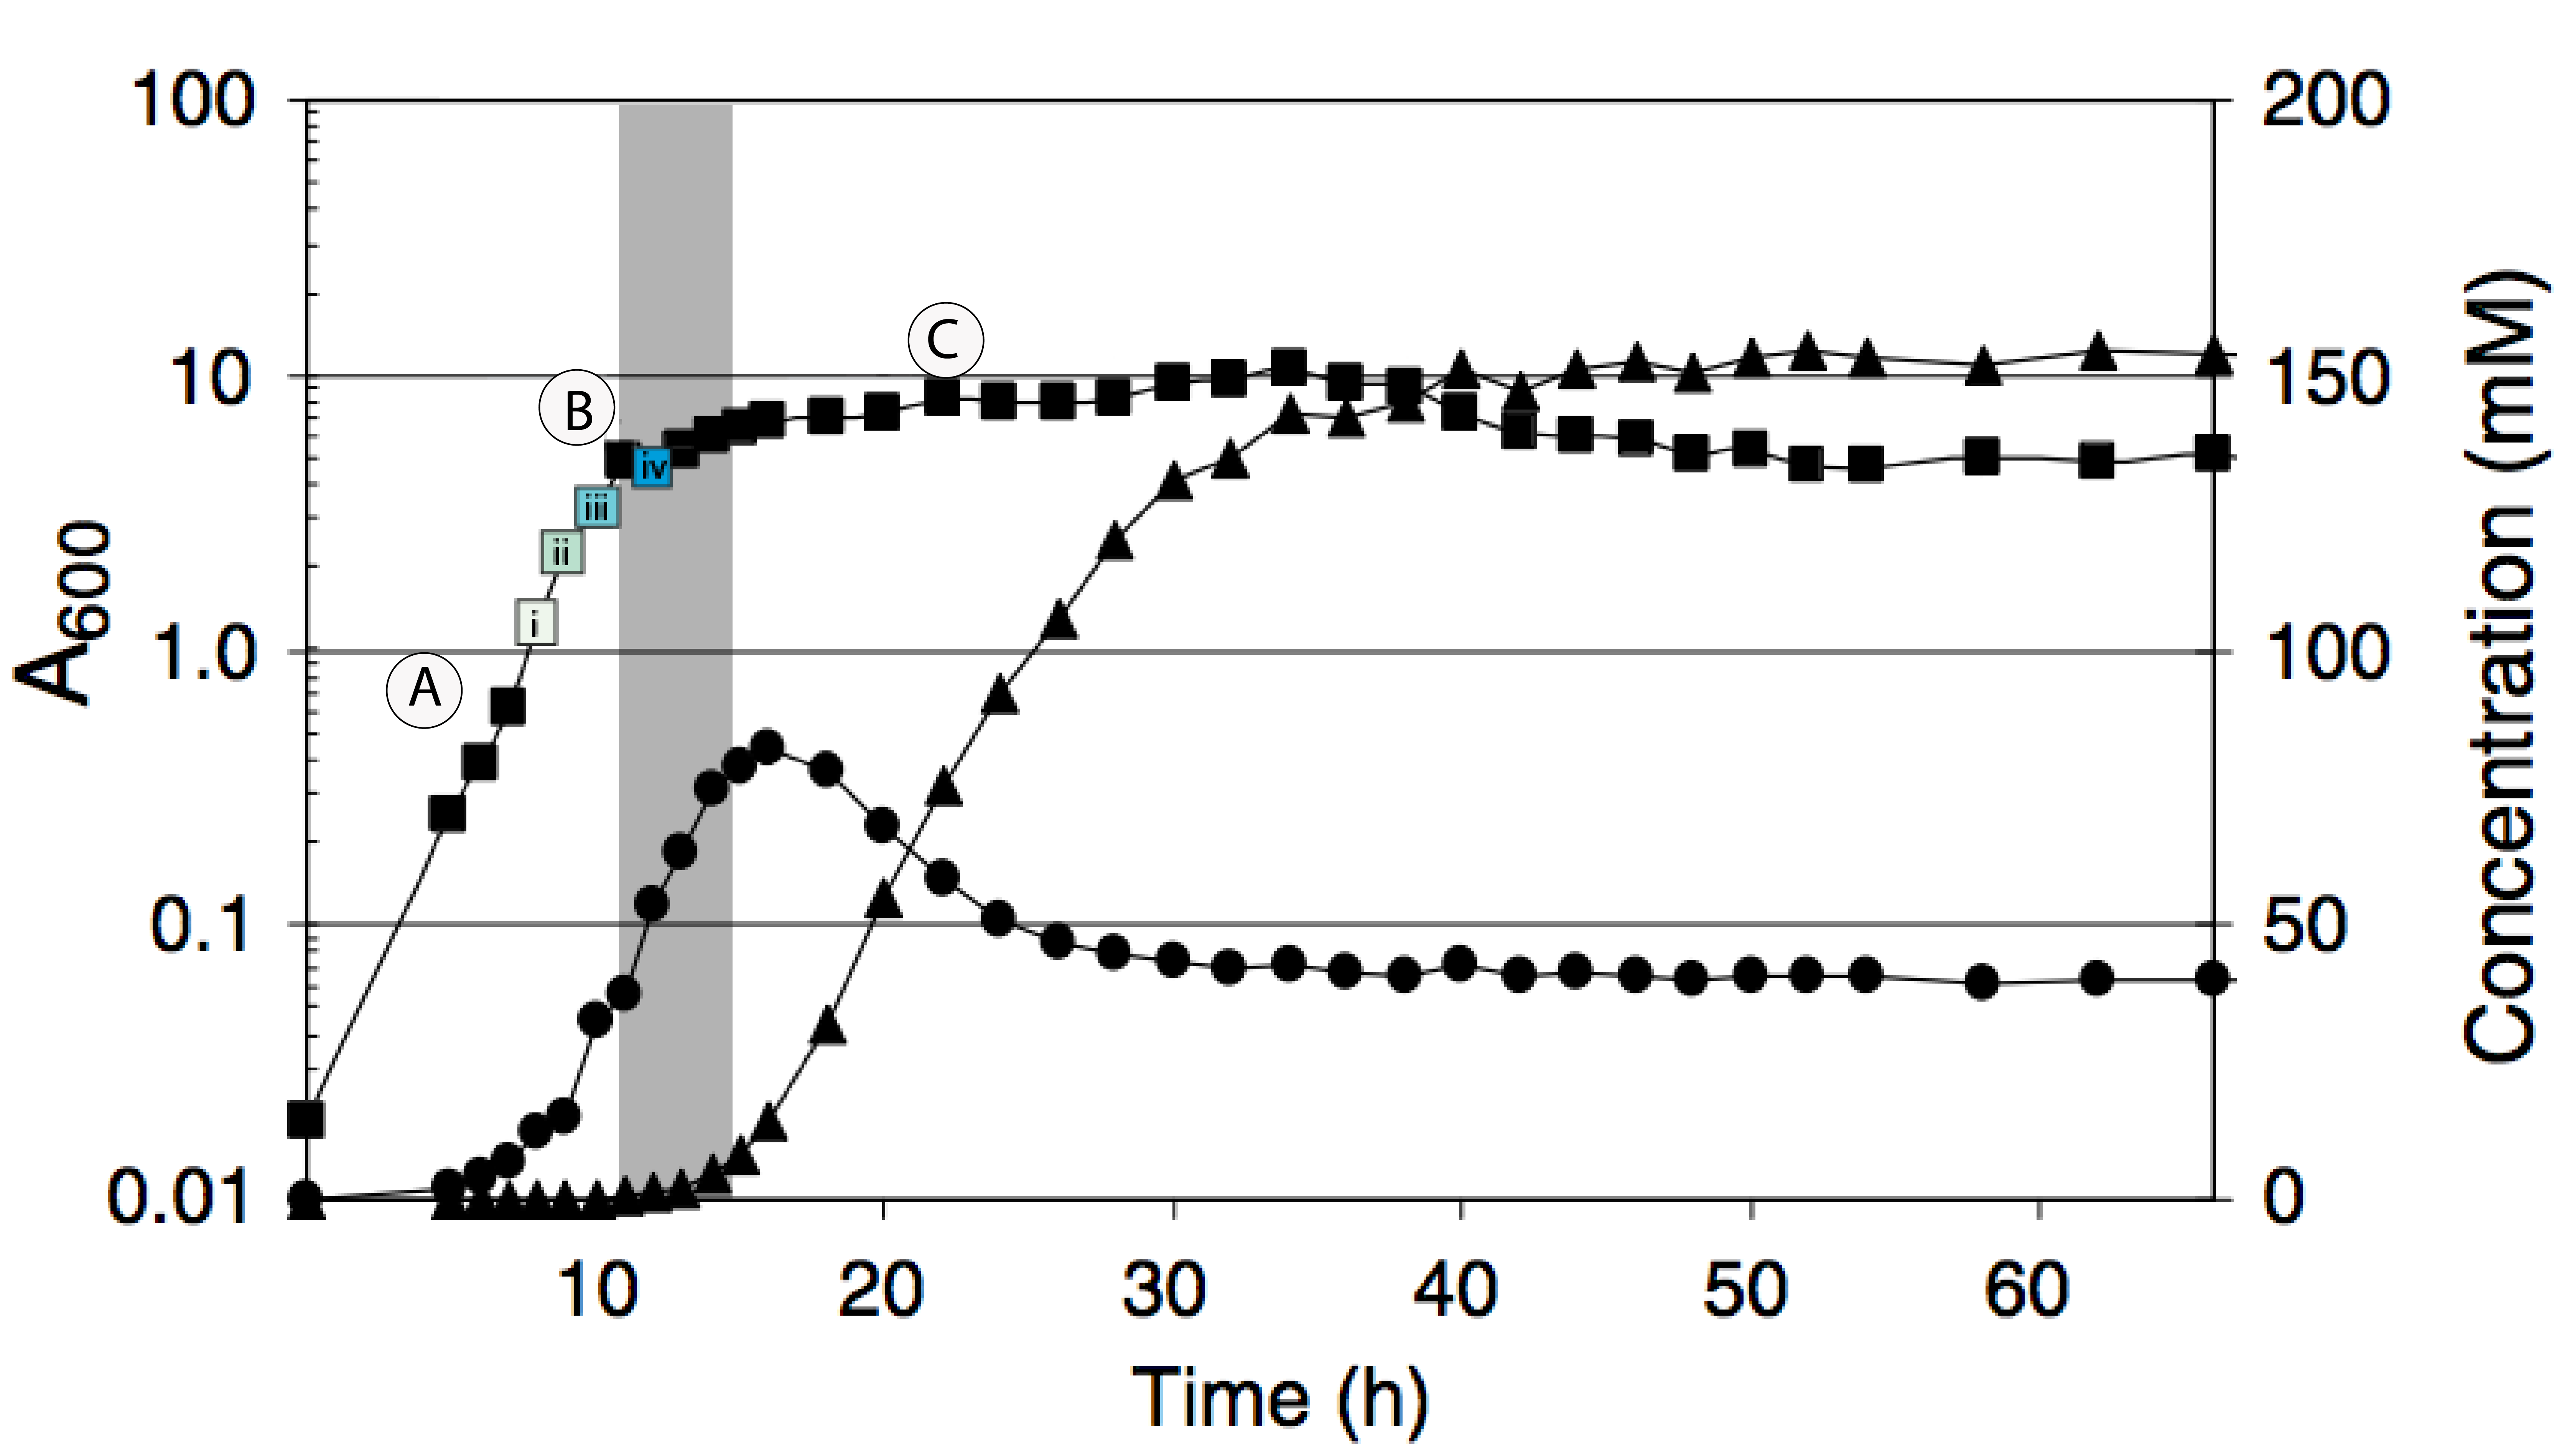
\includegraphics[width=\textwidth,height=3in]{images/Sequencing/Growth_curve.png}
\caption{\textit{C. acetobutylicum} Growth Curve}
\label{fig:1}
This growth curve, adapted from Jones \textit{et al.}(source), illustrates the time points selected for the experimental design. Populations of \textit{C. acetobutylicum} grow through the exponential phase ( A) A_{600} of 1.0), producing carboxylic acids, including butyric acid, during the transition phase (B). Then, the acids are reassimilated and reduced into solvents such as butanol (C). Stress (butyrate, butanol, and control) were assayed in this experiment, in addition to time points 15(i.), 75(ii.), 150(iii.), and 270 minutes (iv.) after synchronization at A_{600} of 1.0. The squares, circles, and triangles represent measurements of A_600, butyrate, and butanol from \textit{C. acetobutylicum} fermentation(source).
\end{figure}

\section{Desirable Data Qualities}
The success of transcript boundary determination with shotgun-strategy sequencing depends on two signals in the dataset, depth and complexity(Nat review assembly). Here depth is defined as the number of reads aligned to a region divided by the size of the region. In the case of a single basepair, this is simply the number of reads aligned to this base. Complexity is the number of unique molecules sequenced by the experiment and can be thought of as the horizontal overlap between aligned reads(Nat review assembly). Algorithmically, the assembly solution's estimates of transcript boundaries improve as depth and complexity increase. Therefore, high depth and complexity are required for successful assembly of the dataset.


In contrast to DNA sequencing, depth in RNA-seq experiments is non-uniform and has a different error profile. The number of reads aligned to a base is a good estimate of its expression. However, the nature of gene expression and sequencing depth is highly variable and non-normal(stats reference). Furthermore, several factors of the experimental procedure result in type I and type II errors, components of the depth signal not addressed in many studies(references, background section). Sequence specific (hexamer (source), GC(source) bias) or technical causes (background antisense(nat compar ssRNAseq), spurious transcription(source??)) raise the variability and background of the depth signal and have no existing bioinformatic solution. Fortunately, other errors such as DNA contamination, RNA degradation, and overabundant sequences (e.g. rRNA) can be addressed with adjustment to laboratory and analytical workflows. Specifically, the quantity of useful data in Illumina-based RNA sequencing of prokaryotes can be maximized by acquiring pure, undegraded RNA and removing ribosomal RNA transcripts. Optimal sequencing depth was the first goal for this study.

While the depth or quantity of data is critical for the shotgun-strategy sequencing approaches, complexity in the data provides overlap between the sequenced fragments, which is required for transcriptome assembly. Most useful assembly algorithms are overlap consensus or de Bruijn graph based, directly relying on the k-mer complexity of the dataset (where k is an integer and a k-mer is a k-length subsequence of a read) to provide significant overlaps to form the graph(Nat assembly review, others). Therefore, a large amount of reads with long horizontally overlapping segments (i.e. complexity) results in a useful graph, which can be traversed by an Eulerian walk. Complexity results from the fragmentation process and the random sampling of these fragments from the library. Complexity is negatively affected by preferential PCR amplification of certain sequences, leading to their over-representation in the final library and dataset. Sequencing complexity is a useful quality for both gene expression and transcriptome assembly studies. A high complexity dataset facilitates transcript boundary identification, especially in the case of low abundance transcripts, and was therefore another goal of this study.

Precision and accuracy of boundary determination relies on both depth and complexity. The probability of sampling critical 5$\prime$ or 3$\prime$ terminal reads from a transcript is a function of the size of the library, the probability of sampling a terminal fragment, and the depth that the library was sequenced. Correct assembly of these reads requires high complexity in the dataset for assembly. Ultra high depth (encode reference) increases the probability of sampling critical reads from low abundance transcripts and terminal reads while providing the required complexity for assembly and boundary determination. Therefore, improving RNA quality and mRNA content while minimizing amplification optimizes both depth and complexity, improving the precision of transcript boundary estimates beyond traditional approaches. With these data qualities in mind, the following RNA processing workflow was established.



\section{Laboratory Workflow}
A protocol was established to optimize library depth and complexity with hybridization and enzymatic steps(\ref{methods:RNA_prep}). After the manipulation stepsthe samples were twice washed with 70\% ethanol, stored as precipitates to minimize degradation, and aliquots were taken for quality control. The quality control procedure consisted of spectrophotometric and electrophoretic analyses to ensure RNA purity and integrity.

\subsection{Quality Control}
After washing with ethanol, the absence of salts, divalent cations, and proteins was assessed through spectrophotometry (methods). These contaminants can cause RNA degradation or adversely affect the enzymatic reactions of RNA manipulation and library construction. Ratios of absorbance ($\sfrac{\SI{260}{\nano\meter}}{\SI{280}{\nano\meter}}$, $\sfrac{\SI{260}{\nano\meter}}{\SI{230}{\nano\meter}}$) are frequently used to describe the purity of nucleic acid samples, due to purine/pyrimidine absorbance maxima at \SI{260}{\nano\meter}. Observed ratios of 2.0 indicated pure RNA, optimal for high depth and complexity RNA-seq. 

\begin{figure}
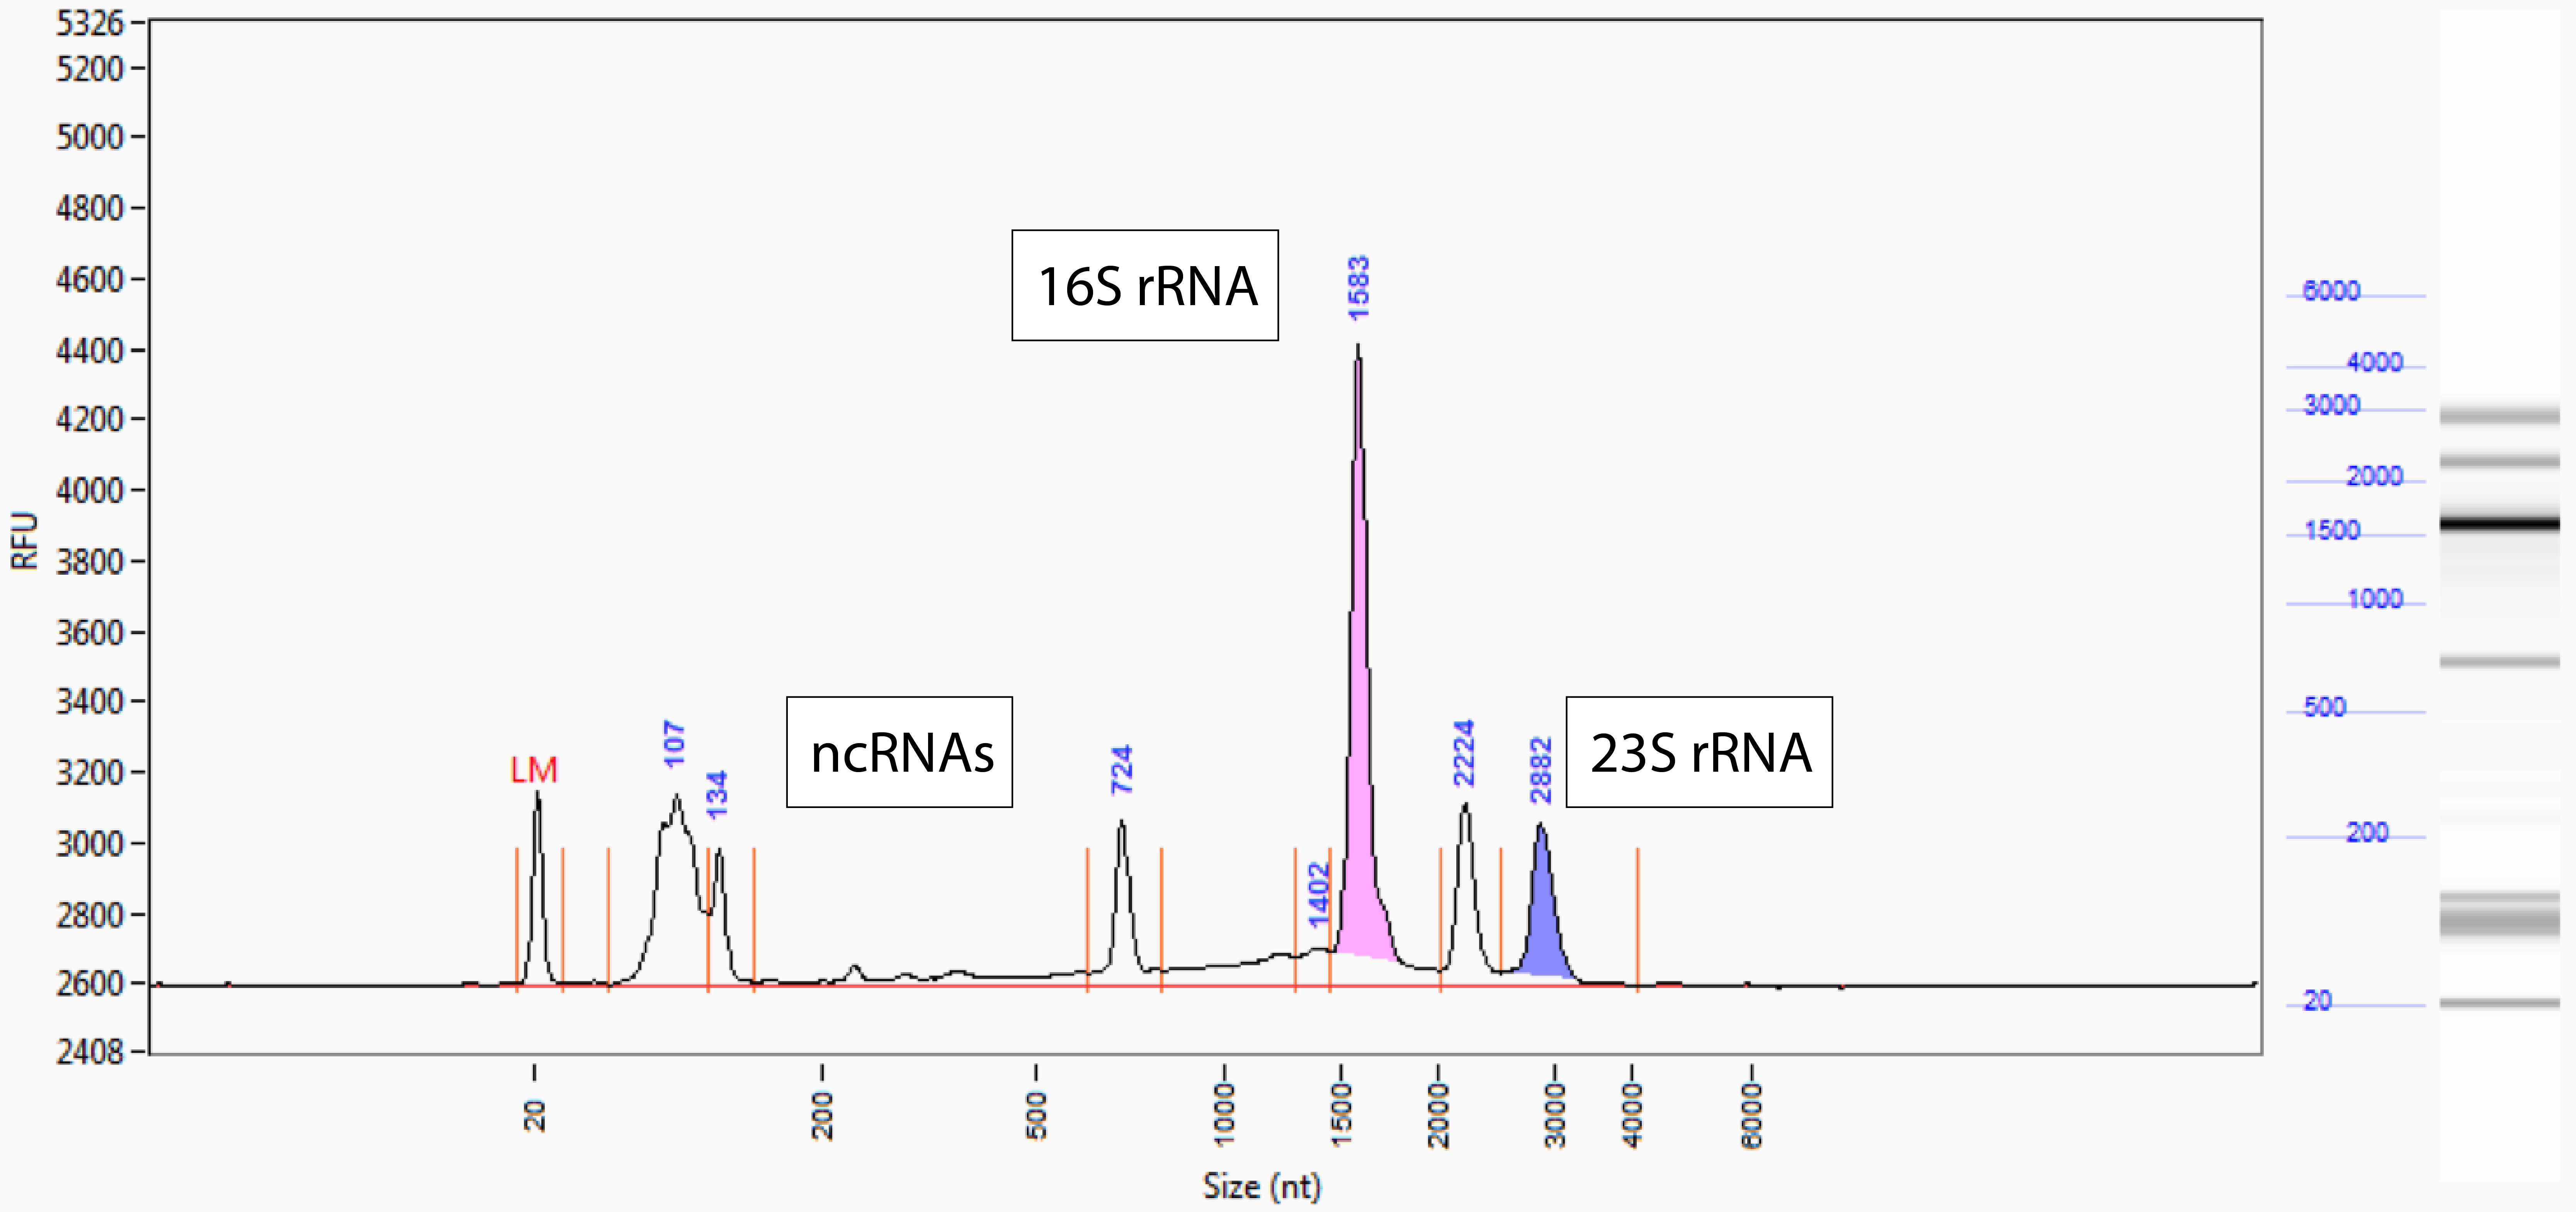
\includegraphics[width=\textwidth,height=3in]{images/Sequencing/RNA-integrity.png}
\caption{RNA Quality}\label{fig:2}
In this electropherogram, dominant and intact rRNA peaks are visible along with a substantial small RNA population, resulting from the miRNeasy kit used for RNA extraction.
\end{figure}

RNA integrity is commonly analyzed by interpreting ribosomal RNA bands obtained with electrophoretic techniques. Specifically, a small peak width of the rRNA electrophoretic bands with little background signal indicates that the RNA high quality (e.g. RNA Integrity Number). A representative electropherogram is shown in \ref{fig:2}. The results indicated that the RNA was undegraded, with sharp peaks for the 16S and 23S rRNA bands. At each QC step (\ref{fig:3}), the RNA had clear pellets, clean spectrophotometric ratios, and the electrophoresis suggested that the RNA were undegraded. The passing samples were then used in subsequent hybridization and enzymatic steps.

\begin{figure}
\hbox to \textwidth{\hfill
\rotatebox{90}{%
\begin{minipage}{\textheight}
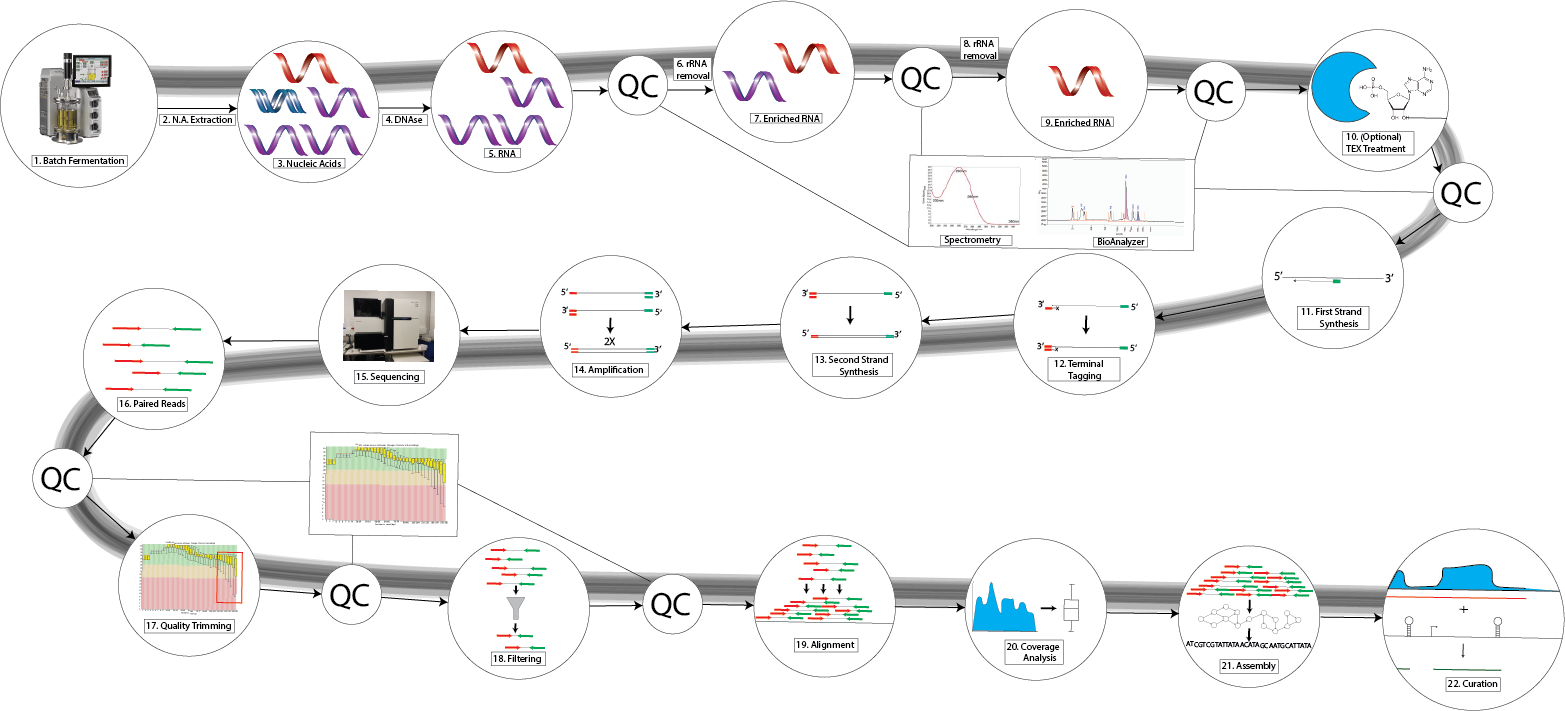
\includegraphics[width=\textheight,height=5in]{images/Sequencing/Workflow.png}
\caption{Laboratory Workflow}\label{fig:3}
The laboratory workflow consisted of mRNA enrichment steps and quality control analyses to ensure RNA quality. Ligation-free library preparation resulted in paired-end Illumina reads for preprocessing, alignment, analysis, and assembly.
\end{minipage}}\hfill}
\end{figure}


\subsection{mRNA/sRNA Enrichment}
High quality sequencing data depended upon enrichment of primary transcripts (mRNAs and sRNAs) and minimization of background signal (e.g. degraded transcripts, DNA) through RNA manipulations(\ref{fig:3}). After extraction, residual DNA was removed with DNAse treatment (Step 4., \ref{fig:3}). Following an initial quality-control checkpoint (QC), ribosomal RNA was removed through a generic hybridization method. After additional QC, the primary transcripts were further enriched with an additional round of rRNA removal. Next, technical replicates of the first biological replicates of 2 times points(75 and 270 minutes) and all stress types (6 total) were treated with a 5$\prime$-phosphate specific exonuclease, which does not degrade primary transcripts. This technique further enriched for primary transcripts and removed rRNA and degradation products. This workflow maximized depth and complexity for the transcripts of interest. These enriched samples were subject to a final QC checkpoint and after clearance used for sequencing.


\section{Data Processing, Alignment, and Coverage Analysis}
The libraries were sequenced paired-end over 6 lanes of an Illumina HiSeq 2500, producing 1.5 billion 75bp reads, averaging 25 million clusters/pairs per library(\ref{app:read_summary}). The reads were then processed through a customized bioinformatic workflow (\ref{methods:data_proc_aln}), first trimming low-quality bases, then filtering ribosomal RNA reads, and finally aligning to the genome (\ref{fig:3}). On average, 97\% of the useful, non-ribosomal reads were aligned to the \textit{C. acetobutylicum} genome(\ref{fig:4}). Of these, 7.75M(83\%) per sample were properly paired, that is, both mates of each pair were in the correct orientation. In total, 458,814,860 perfectly paired reads were produced and then used for subsequent analysis. 

\begin{figure}
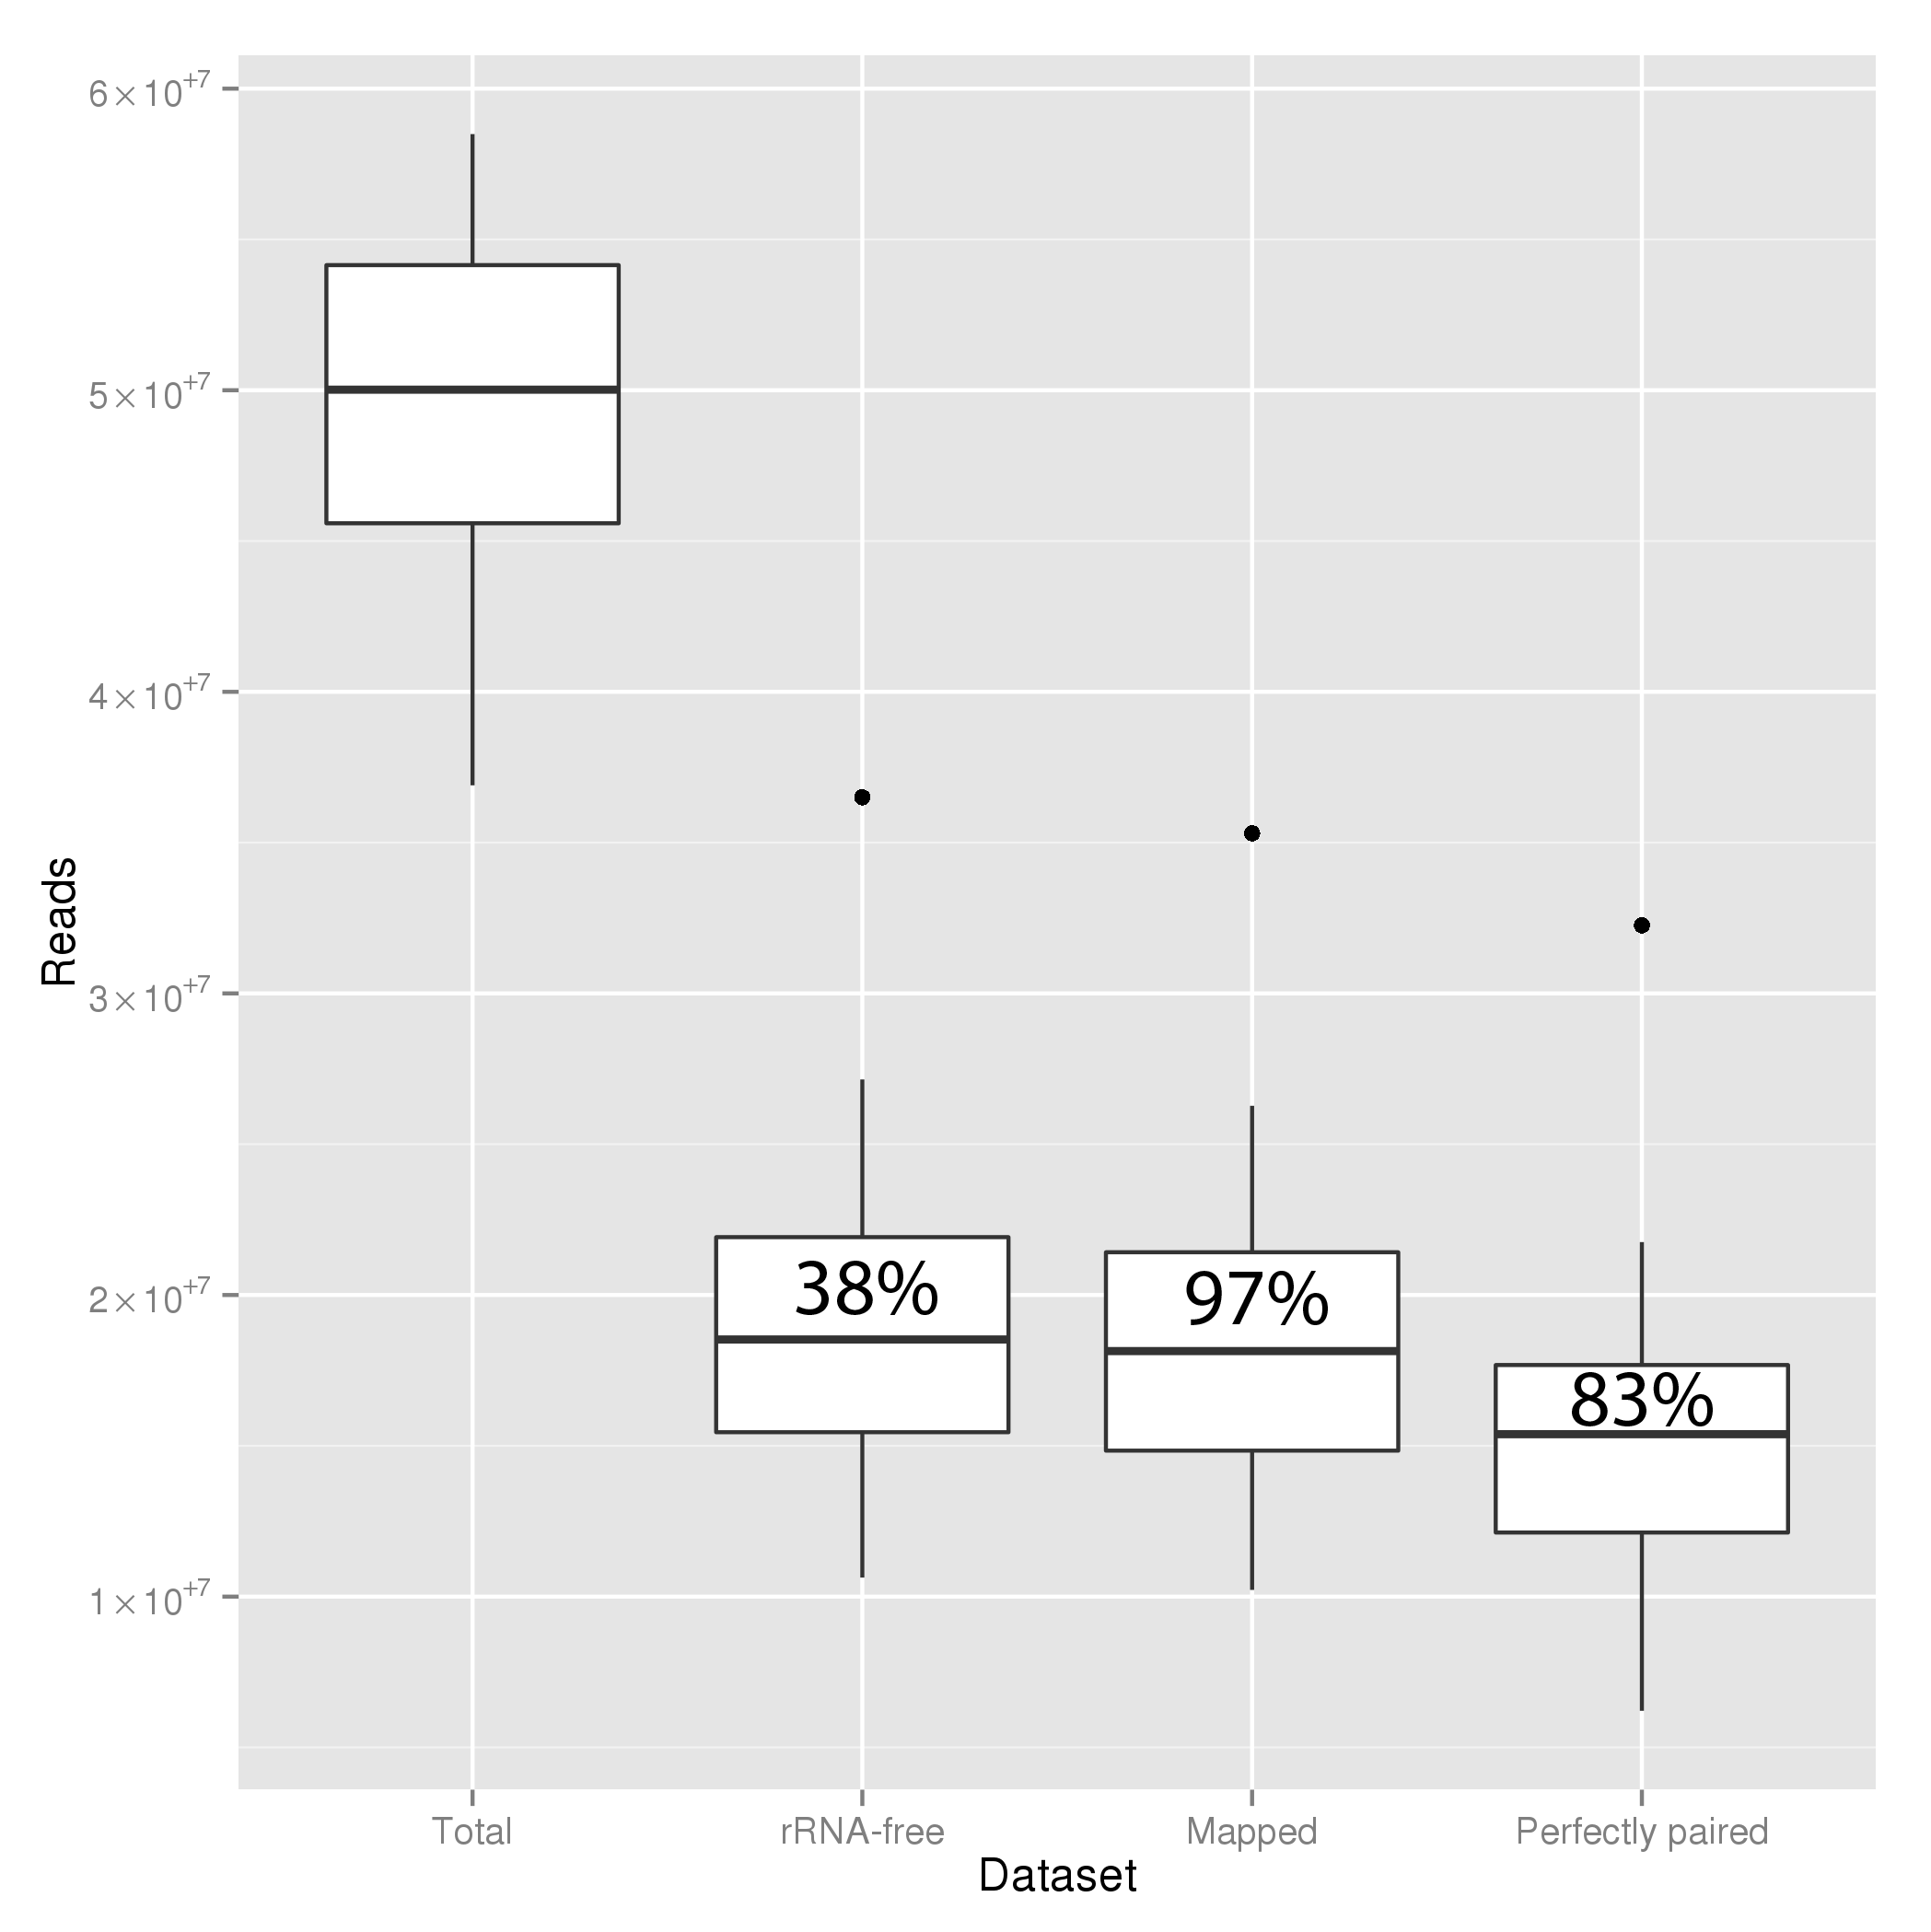
\includegraphics[width=\textwidth,height=4in]{images/Sequencing/Alignment_brief.png}
\caption{Sequence Read Processing and Alignment}\label{fig:4}
An average of 50 million reads (25M clusters/pairs) was produced for each of the 30 libraries. Ribosomal RNA reads were then filtered and the remaining reads were then aligned to the genome. Of these, 83\% were properly paired reads, ideal for transcriptome assembly.
\end{figure}

To understand the depth of sequencing, it was desirable to determine the per-base sequencing depth throughout the genome. Two methods are frequently used to quantify and summarize depth. The first approach is to sum the number of sequenced bases and divide by the estimated size of the transcriptome or genome. The underlying assumption of uniform distribution of reads is not valid for transcriptomic sequencing. The more precise approach is to calculate the number of reads aligned to each base and summarize the distribution with central tendency measures. No single sequencing depth is more significant than another (e.g. 10x vs 9x) and different numbers of reads can be equally effective in different sized genomes. However, the Encyclopedia of DNA Elements (ENCODE) project has released best practice guidelines for RNA-seq projects (Source??) and can be used for benchmarking. 

Heuristically, it seems that a coverage of 100-200 million(M) 100bp paired-end reads is sufficient to detect low abundance transcripts in the 60-140 megabase(Mb) hg19 human transcriptome. This sums to 20-40 gigabases(Gb) of sequencing, 120-660 times the conservative estimate of the size of the human transcriptome. In the case of \textit{C. acetobutylicum}, the maximum possible size of the transcriptome is 8.2Mb, with a realistic estimate of 4-6Mb. With 450M properly-paired reads, 68.7 Gb were sequenced for a much smaller transcriptome, approximately 11-17 thousand times the length of the transcriptome. This estimate suggests that, cumulatively, this study achieves comparable or superior depth than recommended by these guidelines using the first method for depth calculation. 

Using the second method, a median of > 10x coverage per base and per strand was observed for each of the 30 libraries (\ref{fig:5a}). Cumulatively, the median per base coverage is 156x throughout the genome(\ref{fig:5b}). The median depth in truly transcribed regions is greater as shown in the next chapter. Rather, some of the depth described by this distribution(\ref{fig:5b}) was due to previously discussed background signals. Background signal is indeed a pressing concern for RNA-seq (ENCODE source), complicating the determination of transcript boundaries.


\begin{figure}
\begin{center}
\begin{minipage}{.5\textwidth}
\begin{center}
{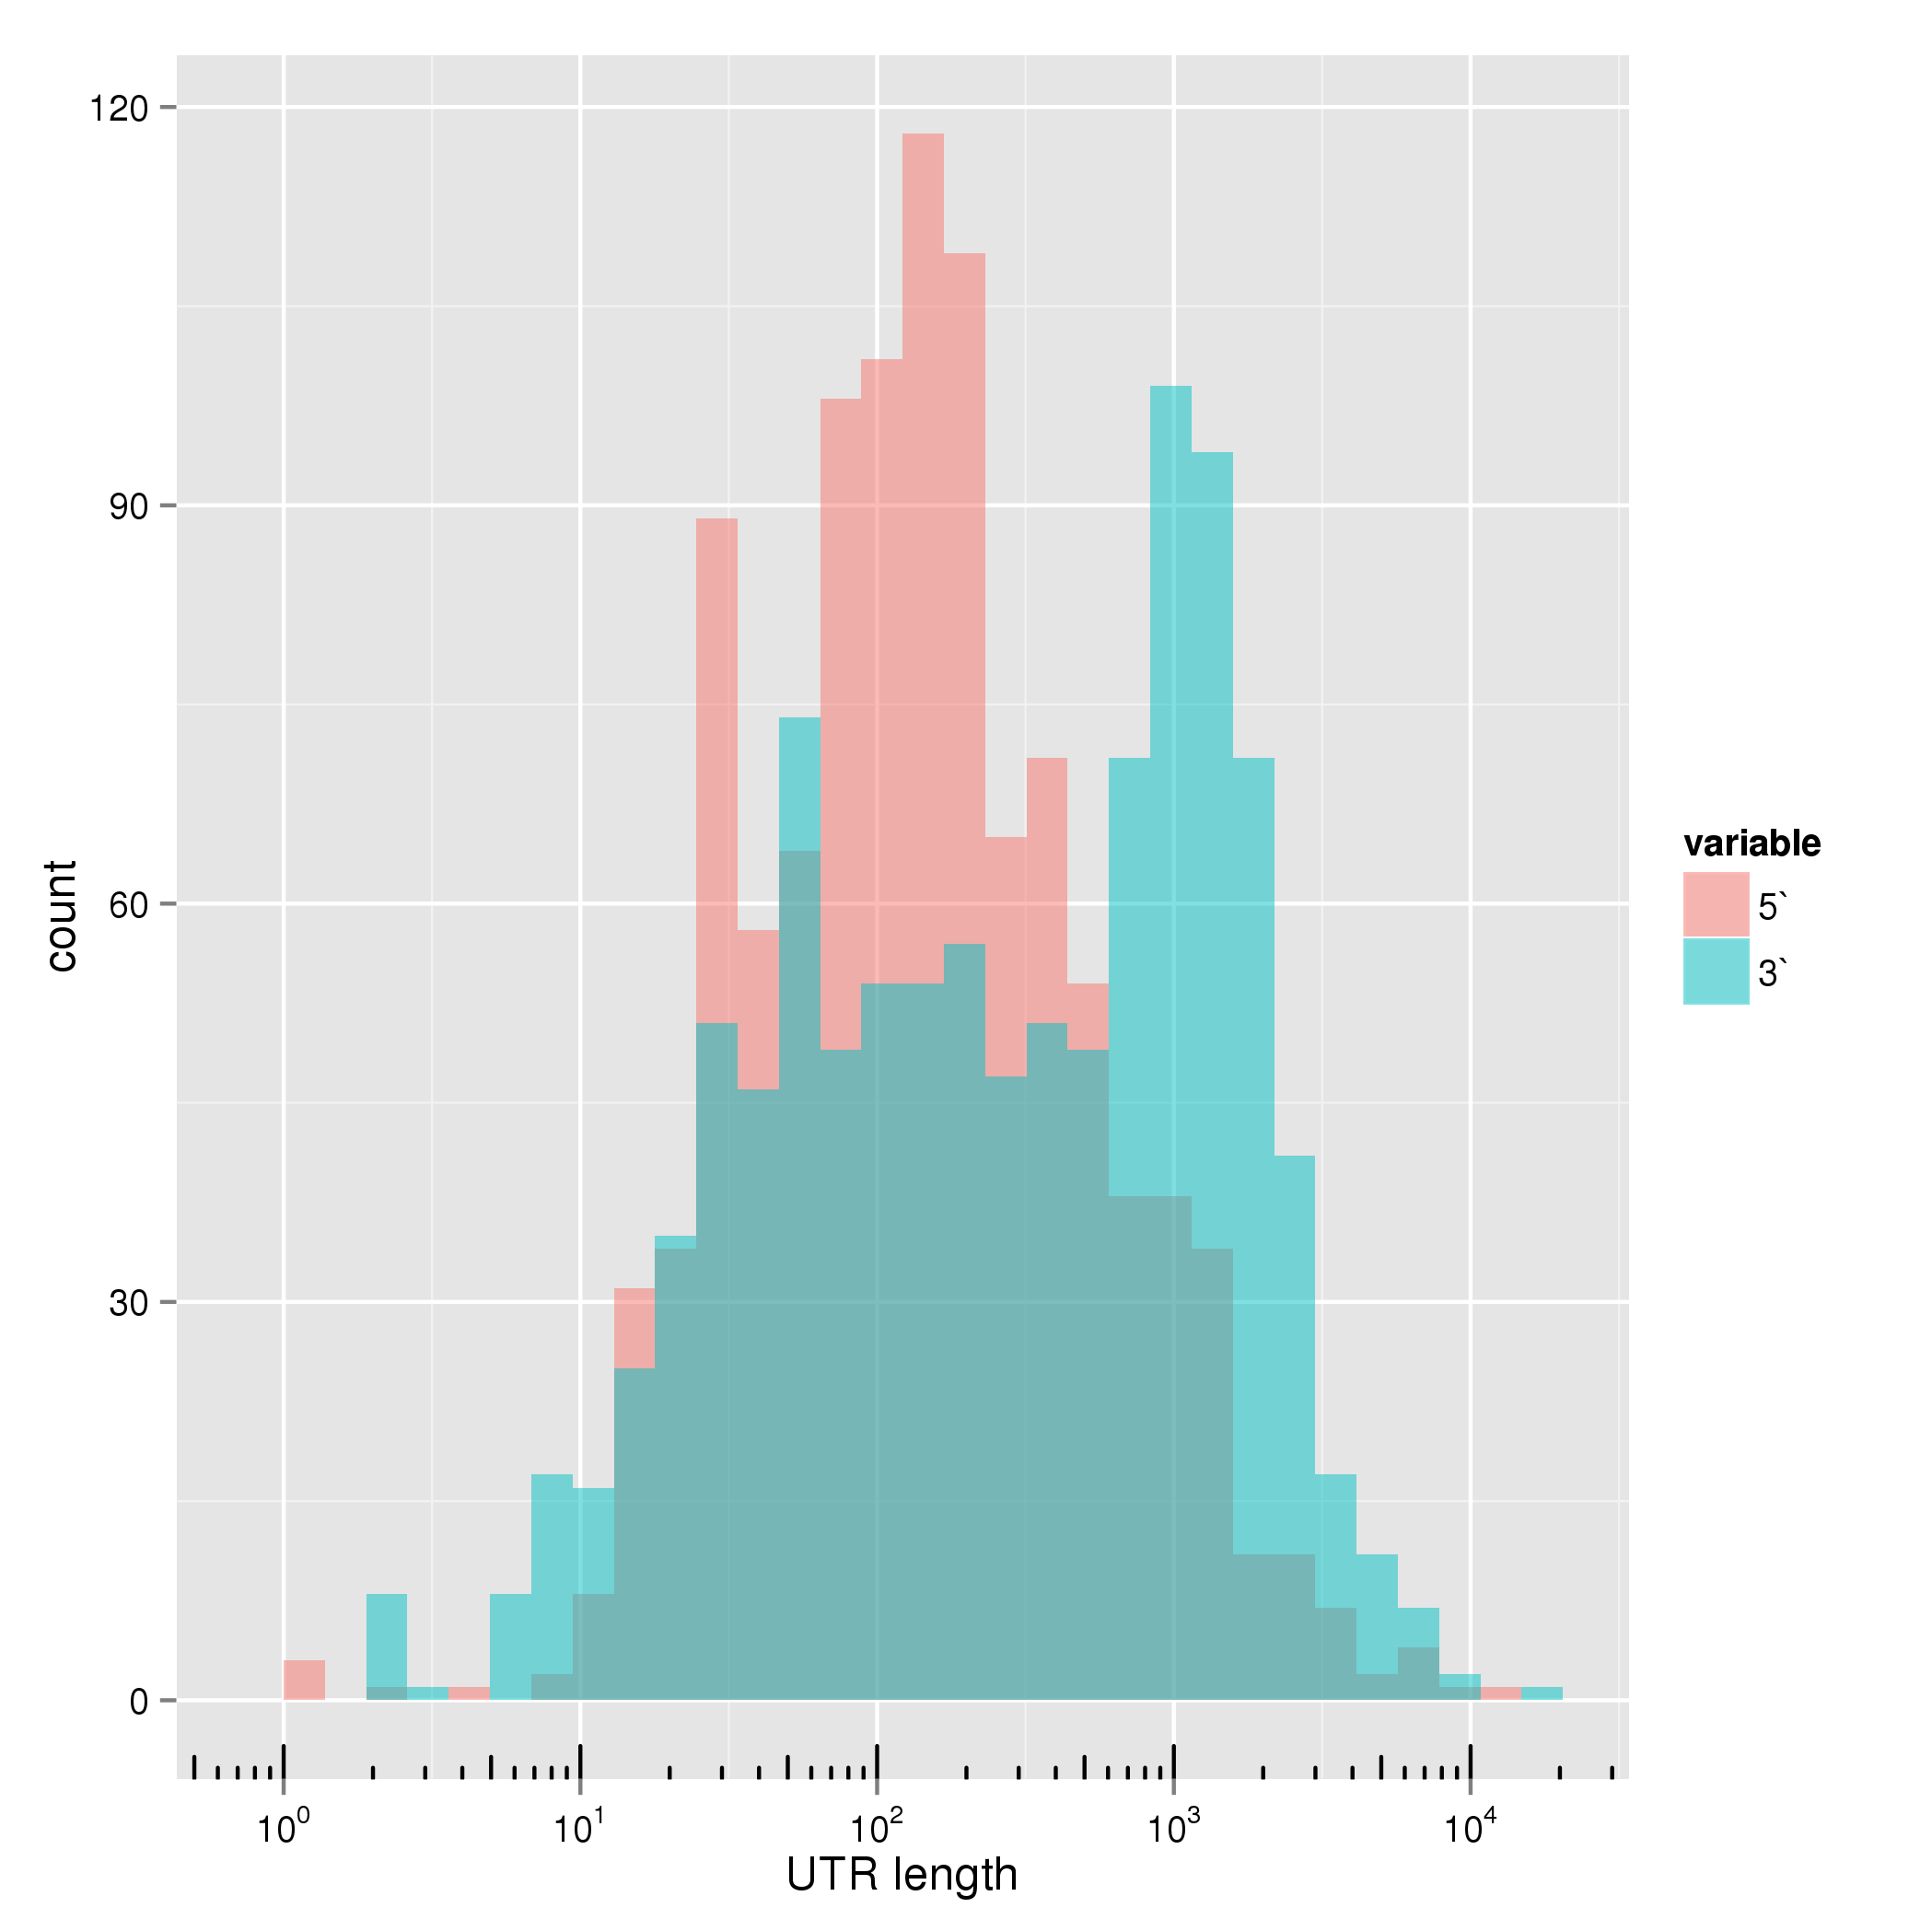
\includegraphics[width=\linewidth,height=3in]{images/Assembly/Summary/futrlength.png}}
\subcaption{5$\prime$ and 3$\prime$ Untranslated Region Length}\label{fig:5a}
\end{center}
\end{minipage}%
\begin{minipage}{.5\textwidth}
\begin{center}
{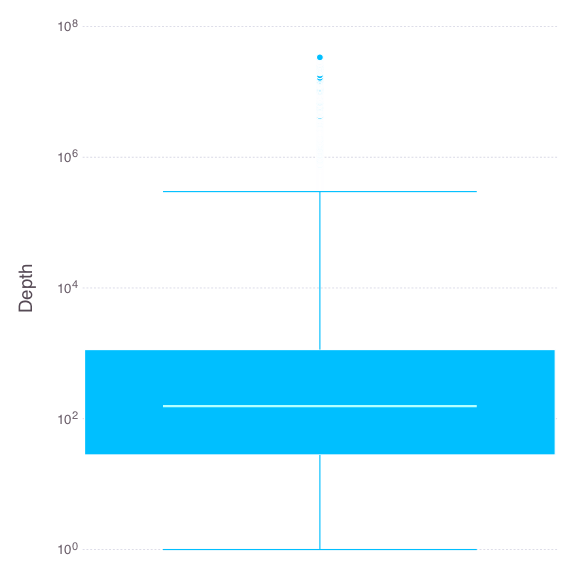
\includegraphics[width=\linewidth,height=3in]{images/Sequencing/Cumulative_depth_boxplot.png}}
\subcaption{Cumulative Depth Distribution}\label{fig:5b}
\end{center}
\end{minipage}
\end{center}
\caption{Coverage Boxplots}
The distribution of coverage throughout the genome from a single library \subref{fig:5a}) is compared to cumulative coverage \subref{fig:5b}), showing high depth has been achieved.
\end{figure}

In summary, the data suggested a successful first aim: a quality RNAseq dataset for subsequent assembly and annotation. The experiment and RNA processing protocol were designed with depth and complexity in mind. Primary transcripts were enriched and contaminants were removed, controlling for RNA purity and integrity after each manipulation. Thirty samples were sequenced over five lanes, resulting in 1.5 billion reads, with 458 million properly-paired reads aligning to the genome. Analysis of the aligned sequences demonstrated consistently high primary transcript enrichment, alignment rates, and sequencing depth. This depth of signal is comparable or superior to many similar studies in prokaryotes and to guidelines for human genome sequencing.



